\chapter{Modelo e implementación}
\pagenumbering{arabic}
Para la realización de este trabajo, se han diseñado y desarrollado una serie de agentes a los que se les ha entrenado para la obtención de un comportamiento de fototaxis, es decir, de
búsqueda y acercamiento a fuentes de luz.

Cada agente esta modelado como un círculo con dos sensores en la parte frontal que permiten recibir lecturas de los diferentes estímulos presentes (ya sean luces u otros agentes) y dos motores opuestos
que permiten que el agente pueda moverse libremente por el espacio, como puede verse
en la figura \ref{fig:figuraMyAgent}. El agente tiene en todo momento una posición en el espacio dada por unas coordenadas (x, y), así como una orientación respecto al eje X. Cada sensor esta separado
60º del eje de orientación del agente. Los sensores tienen un arco de visión de 160º, para representar que el propio cuerpo del agente pueda encontrarse entre el sensor y la luz, evitando las lecturas.

\begin{figure}[H]
	\centering
	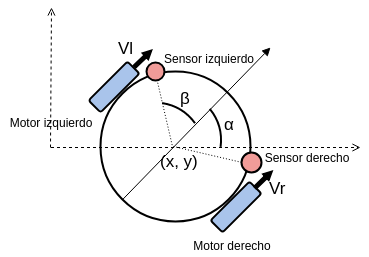
\includegraphics[width=0.6\textwidth,height=6cm]{Imagenes/Agent}
	\caption{Esquema del agente utilizado.}
	\label{fig:figuraMyAgent}
\end{figure}

El movimiento traslacional del agente se calcula a partir de la velocidad lineal ($v$) de su centro de masa (ecuación \ref{eq:VFormula}). El movimiento angular del agente se calcula obteniendo
la velocidad angular ($\omega$) de su centro de masa (ecuación \ref{eq:WFormula}).

\begin{equation} \label{eq:VFormula}
 \centering
 v = \frac{Vr + Vl}{2}
\end{equation}

\begin{equation} \label{eq:WFormula}
 \centering
 \omega = \frac{Vr - Vl}{2R}
\end{equation}

La nueva posición del agente para cada ciclo de ejecución se calcula mediante las ecuaciones (\ref{eq:newXformula}, \ref{eq:newYformula} y \ref{eq:newAformula}), donde $x$ e $y$ representan la posición actual del agente,
$\theta$ representa la orientación actual del agente y $\delta t$ representa el tamaño del tiempo de integración de ciclo.

\begin{equation} \label{eq:newXformula}
 \centering
 x(t + 1) = x(t) + v.cos(\theta).\delta t
\end{equation}

\begin{equation} \label{eq:newYformula}
 \centering
 y(t + 1) = y(t) + v.sin(\theta).\delta t
\end{equation}

\begin{equation} \label{eq:newAformula}
 \centering
 \delta (t + 1) = \delta (t) + \omega .\delta t
\end{equation}

Para los experimentos realizados en este trabajo, el radio del agente siempre se ha tomado como \textbf{4.0}.

\subsection{Plasticidad}
La ultraestabilidad de los agentes desarrollados se ha conseguido dotando a los mismos de mecanismos de plasticidad, que les permiten modificar los valores de algunos de sus atributos internos. En este caso, los agentes pueden
alterar los valores de los pesos $w_{ij}$ de las conexiones entre las neuronas de la red cuando la frecuencia de activación de una neurona es demasiado baja o demasiado alta.

La homeostasis no se encuentra programada explícitamente, pero aparece de forma implícita debido a los mecanismos de evaluación de la evolución genética que recompensan con mejor puntuación a aquellos
agentes que, durante la realización del entrenamiento, han mantenido un mayor número de sus neuronas estables.

La plasticidad de cada conexión esta gobernada por la actividad sináptica de la conexión junto con una regla de plasticidad codificada genéticamente. Estas reglas de plasticidad vienen dadas por las
ecuaciones (\ref{eq:R0plasticityRule}, \ref{eq:R1plasticityRule}, \ref{eq:R2plasticityRule} y \ref{eq:R3plasticityRule}), donde $\Delta w_{ij}$ es el incremento por unidad de tiempo de un determinado peso sináptico ($w_{ij}$), y $z_{i}$ y $z_{j}$ son las frecuencias de
activación de las neuronas presinápticas y postsinápticas respectivamente.

Las reglas de plasticidad se construyen en torno a cuatro parámetros: la frecuencia de aprendizaje ($n_{ij}$), un valor límite ($z_{ij}^{o}$), el grado de facilitación plástica local ($p_{j}$) y
un factor de amortiguación linear que restringe el cambio dentro de los limites establecidos para los valores de los pesos sinápticos ($\delta$).

\noindent
R0: Sin plasticidad:
\begin{equation} \label{eq:R0plasticityRule}
 \centering
 \Delta w_{ij}= 0
\end{equation}
\noindent
R1: Aprendizaje Hebbiano acotado:
\begin{equation} \label{eq:R1plasticityRule}
 \centering
 \Delta w_{ij}= \delta n_{ij} p_{j} z_{i} z_{j}
\end{equation}
\noindent
R2: Potenciación o depresión amortiguadas de la neurona presináptica cuando la eficacia sináptica es muy alta o muy baja:
\begin{equation} \label{eq:R2plasticityRule}
 \centering
 \Delta w_{ij}= \delta n_{ij} p_{j} (z_{i} - z_{ij}^{o}) z_{j}
\end{equation}
\noindent
R3: Potenciación o depresión amortiguadas de la neurona postsináptica cuando la eficacia sináptica es muy alta o muy baja:
\begin{equation} \label{eq:R3plasticityRule}
 \centering
 \Delta w_{ij}= \delta n_{ij} p_{j} z_{i} (z_{j} - z_{ij}^{o})
\end{equation}

El grado de facilitación plástica local ($p_{j}$) se ve incrementado linealmente (hasta un valor máximo de 1) cuando la frecuencia de activación aumenta hasta salirse de sus límites, facilitando
así los cambios plásticos. Cuando la frecuencia de activación entra en sus límites, $p_{j}$ decrece linealmente (hasta un valor mínimo de -1), disminuyendo la facilidad de los cambios plásticos.

El cambio en la conexión sináptica depende del signo de $n_{ij}$, de forma que cada neurona puede actuar de manera independiente facilitando los cambios plásticos en la dirección indicada.

El factor de amortiguación lineal ($\delta$) asegura que los valores de los pesos se mantienen dentro de los límites establecidos para ellos.

El factor de valor límite ($z_{ij}^{o}$) depende linealmente del valor actual del peso que se está actualizando plásticamente, por lo que es calculado en cada modificación.

Los pesos son actualizados cada iteración (si precede, dependiendo de su regla de plasticidad) a partir de la ecuación \ref{eq:WeightUpdate}.
\begin{equation} \label{eq:WeightUpdate}
 \centering
 w_{ij}(t+1) = w_{ij}(t) + \Delta w_{ij}
\end{equation}

\section{Agentes}
Durante la realización de este trabajo se han diseñado e implementado tres tipos de agentes distintos. En esta sección se describe cada uno de ellos exponiendo la estructura de la red neuronal que actúa de controlador
y las diferencias entre los controladores de cada agente.
\subsection{Agente 0: agente sin comportamiento social}
Este primer agente fue diseñado e implementado como punto de partida para probar tanto las funciones de evolución como el correcto funcionamiento de los sensores, motores, plasticidad y del comportamiento de fototaxis
que sería utilizado posteriormente en los agentes con habilidades sociales.

El Agente 0 no cuenta con habilidades sociales. Su comportamiento se centra unicamente en la fototaxis, por lo que se acercará a las luces y se mantendrá cerca de ellas.

\subsubsection{Controlador}
El controlador de este agente consiste en una CTRNN de 4 neuronas completamente interconectadas entre sí y autoconectadas (conectadas con todas las demás y con ellas mismas). Como puede verse en la figura \ref{fig:a0Controller},
las neuronas 1 y 2 estan conectadas a los sensores luminosos y son las encargadas de recibir las mediciones y procesarlas. Las neuronas 3 y 4 estan conectadas a los motores, y sus salidas se convierten en la velocidad de los
motores, que permite al agente moverse libremente.

\begin{figure}[H]
	\centering
	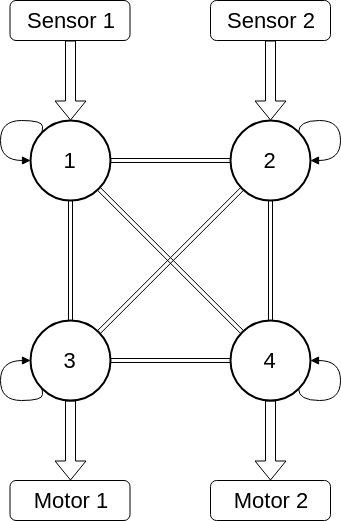
\includegraphics[width=0.4\textwidth,height=7cm]{Imagenes/Agent0Controller}
	\caption{Esquema de la estructura del controlador del Agente 0.}
	\label{fig:a0Controller}
\end{figure}

\subsection{Agente 1: agente colectivo según (Nombre del tio)}
Este agente, al igual que el Agente 0, esta diseñado para seguir un comportamiento de fototaxis, pero además cuenta con habilidades sociales para interactuar con el resto de agentes. Las capacidades sociales del agente se han diseñado
e implementado basandose en la teoría de (Nombre del tio), en la que defiende su creencia de que las habilidades cerebrales de los seres vivos pueden interpretarse como módulos independientes que se entrenan por separado. Es decir, que
el comportamiento social del agente se encuentra aislado del comportamiento de fototaxis del mismo y sus evoluciones son independientes.

El agente obtiene lecturas de los mismos sensores usados para la fototaxis, sobre las posiciones del resto de agentes que puede ver, pero estas lecturas son procesadas por una red independiente y por tanto no conectada al resto de la red.

\subsubsection{Controlador}
El controlador de este agente es similar al del Agente 0, una red CTRNN de 4 neuronas completamente interconectadas. Aunque al contar con habilidades sociales, se ha añadido una capa independiente de 2 neuronas que será la encargada
de procesar las lecturas de los sensores sobre las posiciones de los agentes y de transmitir la señal adecuada a los motores del agente. Como puede verse en la figura \ref{fig:a1Controller}, las neuronas 1 y 2 estan conectadas a los
sensores y se encargan de recibir mediciones de luz y de procesarlas. Las neuronas 5 y 6 estan conectadas a los motores, igual que en el Agente 0. Las neuronas 3 y 4 se encargan de procesar las señales de los sensores sobre el posicionamiento
del resto de agentes, procesarlas y transmitir su salida a los motores. Los motores juntan las salidas de las neuronas 3, 4, 5 y 6 para generar una velocidad.

\begin{figure}[H]
	\centering
	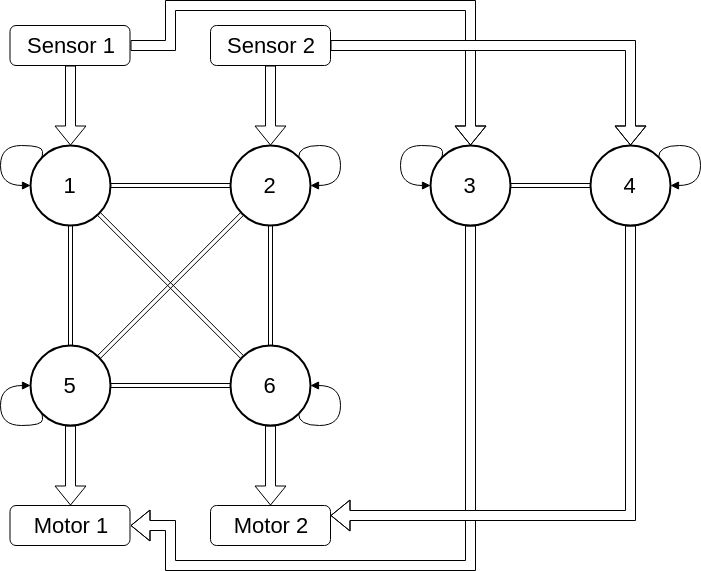
\includegraphics[width=0.6\textwidth,height=7cm]{Imagenes/Agent1Controller}
	\caption{Esquema de la estructura del controlador del Agente 1.}
	\label{fig:a1Controller}
\end{figure}

\subsection{Agente 2: agente colectivo según (Nombre del tio)}
El controlador de este agente es una extensión del controlador del Agente 0. A la red CTRNN de 4 neuronas se le han añadido 2 neuronas más, las cuales estan conectadas a los sensores y se encargaran de procesar las mediciones sobre el posicionamiento
del resto de agentes. La diferencia con el Agente 1 es que estas dos neuronas extra estan interconectadas completamente con el resto de la red, no son independientes. Esta implementación consiste en la teoría de (nombre del señor), que defiende que
las capacidades cerebrales de los seres vivos pueden aprenderse y evolucionar en momentos diversos de su vida, pero esta evolución afecta al resto de las neuronas haciendolas cambiar también. Por tanto, en el Agente 2, el comportamiento social no se
encuentra aislado del comoportamiento de fototaxis.

\subsubsection{Controlador}
El controlador de este agente es similar al del Agente 1, salvo porque la cada extra de 2 neuronas no se encuentra aislada del resto, sino mezclada con el resto. Como puede verse en la figura \ref{fig:a2Controller}, las neuronas 1 y 2 estan conectadas
a los sensores y se encargan de recibir mediciones de luz y de procesarlas. Las neuronas 3 y 4 estan conectadas a los sensores y se encargan de procesar las señales de los sensores sobre el posicionamiento del resto de agentes, pero se encuentran completamente
interconectadas con el resto de neuronas. Las neuronas 5 y 6 generan las salidas que los motores convierten en velocidades.

\begin{figure}[H]
	\centering
	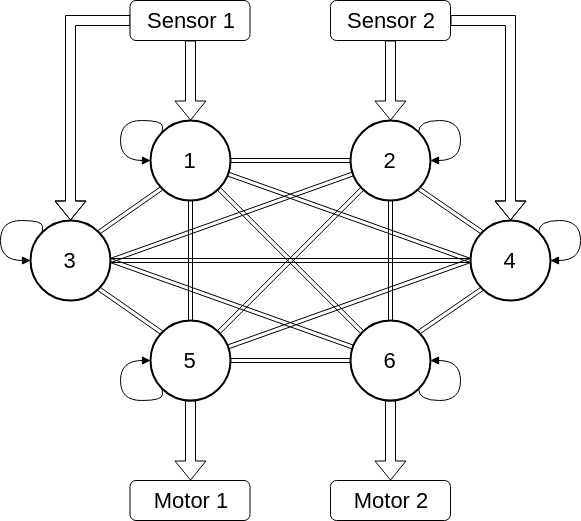
\includegraphics[width=0.5\textwidth,height=7cm]{Imagenes/Agent2Controller}
	\caption{Esquema de la estructura del controlador del Agente 1.}
	\label{fig:a2Controller}
\end{figure}

\section{Evolución}
Para la evolución de los tres tipos de agentes anteriormente descritos se ha implementado un algoritmo genético. El algoritmo es común para los tres agentes, pero algunas de las funciones varían entre los tres tipos para adaptarse a sus estructuras, características y
objetivos propios. De forma común, la estructura del algoritmo es la siguiente:
\begin{enumerate}
\item{Se crea una población inicial de agentes candidatos a ser solución. Los valores de los atributos de estos agentes son completamente aleatorios. Constituyen la primera generación.}
\item{Se evalúan los agentes de la poblacion inicial aplicándoles la función fitness. Se obtiene como resultado un valor de fitness para cada agente de la primera generación.}
\item{Se comprueba si algun agente ha alcanzado un valor fitness lo suficientemente alto como para darlo por entrenado y así finalizar el experimento.}
\item{Si no se encuentra un agente con un valor fitness satisfactorio se procede a crear otra generación.}
\item{Se aplica la función de selección a la generación anterior, obteniendo una nueva población de agentes.}
\item{Se aplica la función de recombinación (\textit{crossover}) sobre la nueva población para generar nuevos agentes.}
\item{Se aplica la función de mutación sobre los agentes para crear pequeñas variaciones sobre los mismos que den más variedad a la generación.}
\item{Se evalúa esta nueva generación de agentes aplicándoles la función fitness. Se obtiene como resultado un valor de fitness para cada agente de esa nueva generación.}
\item{Volvemos al punto número 3.}
\end{enumerate}

\subsection{Codificación de los agentes}
Cada agente candidato es codificado como un vector que contiene cada uno de sus atributos. El Agente 0 se codifica como un vector de 46 componentes formado por 42 componentes reales y 4 componentes enteras, como puede verse en la figura \ref{fig:vector0}.

\begin{figure}[H]
	\centering
	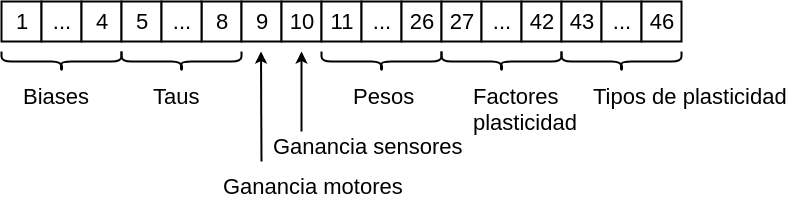
\includegraphics[width=1.0\textwidth,height=4cm]{Imagenes/vector0}
	\caption{Representación codificado de un cromosoma que representa un agente de tipo 0.}
	\label{fig:vector0}
\end{figure}

Los agentes de tipo 1 y 2 estan formados por 6 neuronas, a diferencia de los agentes de tipo 0 que están compuestos por 4 neuronas. Esto hace que el vector de un Agente 1 o de un Agente 2 este formado por 92 elementos, siendo 86 de ellos reales
y 6 enteros, como puede verse en la figura \ref{fig:vector12}

\begin{figure}[H]
	\centering
	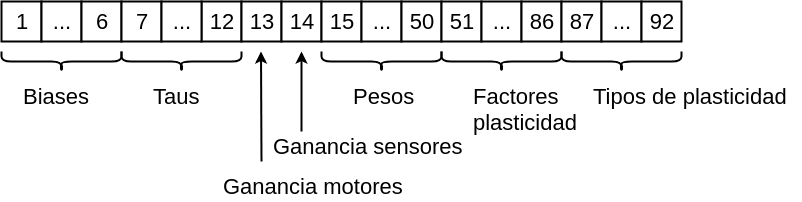
\includegraphics[width=1.0\textwidth,height=4cm]{Imagenes/vector12}
	\caption{Representación codificado de un cromosoma que representa un agente de tipo 1 o 2.}
	\label{fig:vector12}
\end{figure}

Todas las componentes reales de los agentes codificados estan formadas por valores entre [0, 1], los cuales serán escalados a sus rangos establecidos a la hora de evaluar el agente. Las componentes enteras estan formadas por valores del 0 al 3, y
representan los tipos de plasticidad nombrados en el apartado de plasticidad de este documento.

\subsection{Creación de la población inicial}
Para la creación de la población inicial se llama $N$ veces a la función de creación de candidato. Esto da como resultado una población de candidatos aleatorios que constituyen la primera generación.

Se ha seleccionado un tamaño de población inicial ($N$) de \textbf{60} candidatos. Este tamaño se mantiene para el resto de las poblaciones de las siguientes generaciones.

\subsection{Función de selección}
La función de selección es la encargada de elegir los candidatos que serán utilizados para engendrar una nueva generación. Existen muchas formas de seleccionar estos candidatos (de manera aleatoria, los $k$ mejores, los $k$ peores, etc.). En este caso
se ha elegido utilizar la llamada "selección por torneo". Este tipo de selección consiste en elegir de manera aleatoria un número determinado de candidatos de entre la población inicial para "participar en el torneo", el ganador del torneo es el candidato
con mejor fitness de entre los participantes, el cual es seleccionado para engendrar la nueva generación. El torneo se repite hasta que se han elegido ganadores suficientes como para formar una nueva generación.

Se ha elegido este tipo de selección ya que, por una parte selecciona a aquellos candidatos de la generación actual que mejor fitness han conseguido (quedándote con los mejores), mientras que permite que candidatos menos buenos puedan ser también elegidos como ganadores
(por ejemplo, si los participantes elegidos aleatoriamente son aquellos con peores valores de fitness). El permitir que no solamente los candidatos mejores engendren dota de cierta riqueza al algoritmo genético, permitiendo explorar un mayor abanico de posibilidades
que, quedandonos solo con los mejores, no sería posible explorar.

En nuestro algoritmo genético, el número de participantes en los torneos se ha fijado en \textbf{10} candidatos.

\subsection{Función de recombinación}
La función de recombinación o \textit{crossover} se encarga de crear nuevos individuos a partir de los candidatos seleccionados con la función de selección. En nuestro caso, esta recombinación se aplica con una probabilidad del \textbf{50\%}. En ella se eligen dos candidatos aleatorios de la nueva
generación y se aplica el llamado "\textit{crossover} uniforme". En este tipo de recombinación, para cada componente del vector de componentes, los dos candidatos elegidos intercambian sus valores con una cierta probabilidad. El resultado son dos nuevos candidatos formados por componentes de los
elegidos.

En nuestro caso, la probabilidad de que los dos candidatos elegidos intercambien el valor de una componente es del \textbf{0.5}.

\subsection{Función de mutación}
La función de mutación se encarga de aplicar un cierto nivel de aleatoriedad en los candidatos, dando lugar a una mayor riqueza de individuos y una mayor amplitud de resultados posibles. En nuestro caso se ha optado por una mutación básica, la cual se da con una probabilidad del \textbf{50\%}.
La mutación consiste en recorrer el vector de componentes del candidato elegido para mutar, generando un nuevo valor (dentro de sus rangos establecidos) aleatorio para cada componente con una cierta probabilidad.

En nuestro caso, la probabilidad de generar un nuevo valor para una componente real es del \textbf{0.5}, mientras que para una componente entera es del \textbf{0.1}.

\section{Simetría}
Las redes CTRNN que actúan como controladores de los agentes cuentan con simetría en las ganancias de los motores y los sensores. Esto quiere decir que ambos motores comparten el mismo valor para la ganancia y que ambos sensores
comparten el mismo valor para la ganancia.

\section{Parametros y rangos}
Para todos los agentes anteriormente descritos, los rangos establecidos para sus variables internas pueden verse en la tabla \ref{table:tablaValoresParametros}.
\begin{table}[H]
\centering
\begin{tabular}{l|l|c|c}
\textbf{Parametro} & \textbf{Descripción}          & \multicolumn{1}{l|}{\textbf{Valor mínimo}} & \multicolumn{1}{l}{\textbf{Valor máximo}} \\
\textit{$\tau_{i}$}       & Constante de decaimiento      & 0.4                                        & 4.0                                       \\
\textit{$\theta{i}$}      & Bias                          & -3.0                                       & 3.0                                       \\
\textit{Gain}      & Ganancia motora y sensora     & 0.1                                        & 10.0                                      \\
\textit{$w_{ij}$}      & Peso de la conexión sináptica & -10.0                                      & 10.0                                      \\
\textit{$n_{ij}$}     & Ritmo de plasticidad          & -0.9                                       & 0.9
\end{tabular}
\caption{Rango de valores para los parámetros de la red}
 \label{table:tablaValoresParametros}
\end{table}
